\chapter{基于深度学习的算式识别算法}
\section{基于统计直方图的算式分割算法}
为了检查算式正确与否,需要识别出算式中的每一个字符,本文的思路是识别出每一个字符后,拼接成算式然后判断是否正确,并且本文训练模型的数据集是单个字符,只能识别含有单个字符的图片。因此,把算式切分成字符就十分必要。 
\par
读取图像后首先对图片进行伽马变换,修正相机过曝和曝光不足的图片,增加图片的对比度。使用手机随手拍出的照片经常是光照不均匀的,对图像的二值化操作和投影直方图的计算会产生很大干扰。所以需要根据背景像素来确定阈值,使用局部阈值自适应算法来实现图片二值化。 本文使用OpenCV的adaptiveThreshold函数将灰度图二值化,自适应方法使用高斯分布加权和计算局部阈值,二值化类型选择THRESH\_BINARY,大于局部阈值的像素点设为最大值。

\[ r(x,y)= \begin{cases}
255,\quad s(x,y)>t(x,y) \\
0,\quad others
\end{cases} \]
\par
s(x,y)是当前点的像素值,t(x,y)是区域内的高斯均值减去函数的最后一个参数double C的结果,r(x,y)是当前点二值化后的像素值。
\par
获取二值化的图像后,利用字符间隔的特点, 把二维的图像矩阵先按行统计,把二维的矩阵缩减成一列,得到每一行的投影直方图,设定阈值和得到的直方图比较可以得到每一行算式的上边沿和下边沿,然后就可以把水平方向的一行算式切割出来;获取单个算式后,把二维的图像矩阵按列统计,缩减成一行,把设定的阈值与缩减好的矩阵比较获取每一个字符的左边缘和右边缘。在切割图片获取单个字符图片的同时记录它们在原图上的位置和所在算式的序号。
\par
通过上一步一张图片上的算式被分割成了单个字符,由于是紧贴着边缘剪切,图片的长宽比有可能比较极端,不能直接输入到模型中识别。即使根据图片的长宽比,进行上下和左右填充,在一行算式排列倾斜时,也会存在图片内的字符被缩放的过小,导致无法正确识别的现象。本文采取获取字符紧贴边缘的图片后再填充的策略,首先获取图像中像素不为零的点,然后找到包含这些点的最小矩形,根据找到的矩形切割图片获的字符紧贴边缘的图片,如果图片的长和宽均不足原图的1/10或不存在最小矩形,则认为该字符为图片中的干扰,放弃识别这个字符。最后根据图片的长宽差进行填充,调整图片大小为28*28。将图片导入模型识别出对应的字符后,拼接成算式字符串,然后判断算式是否正确,根据判断的结果,在原图上做出对应的标记。
\begin{figure}[h!]
	\centering
	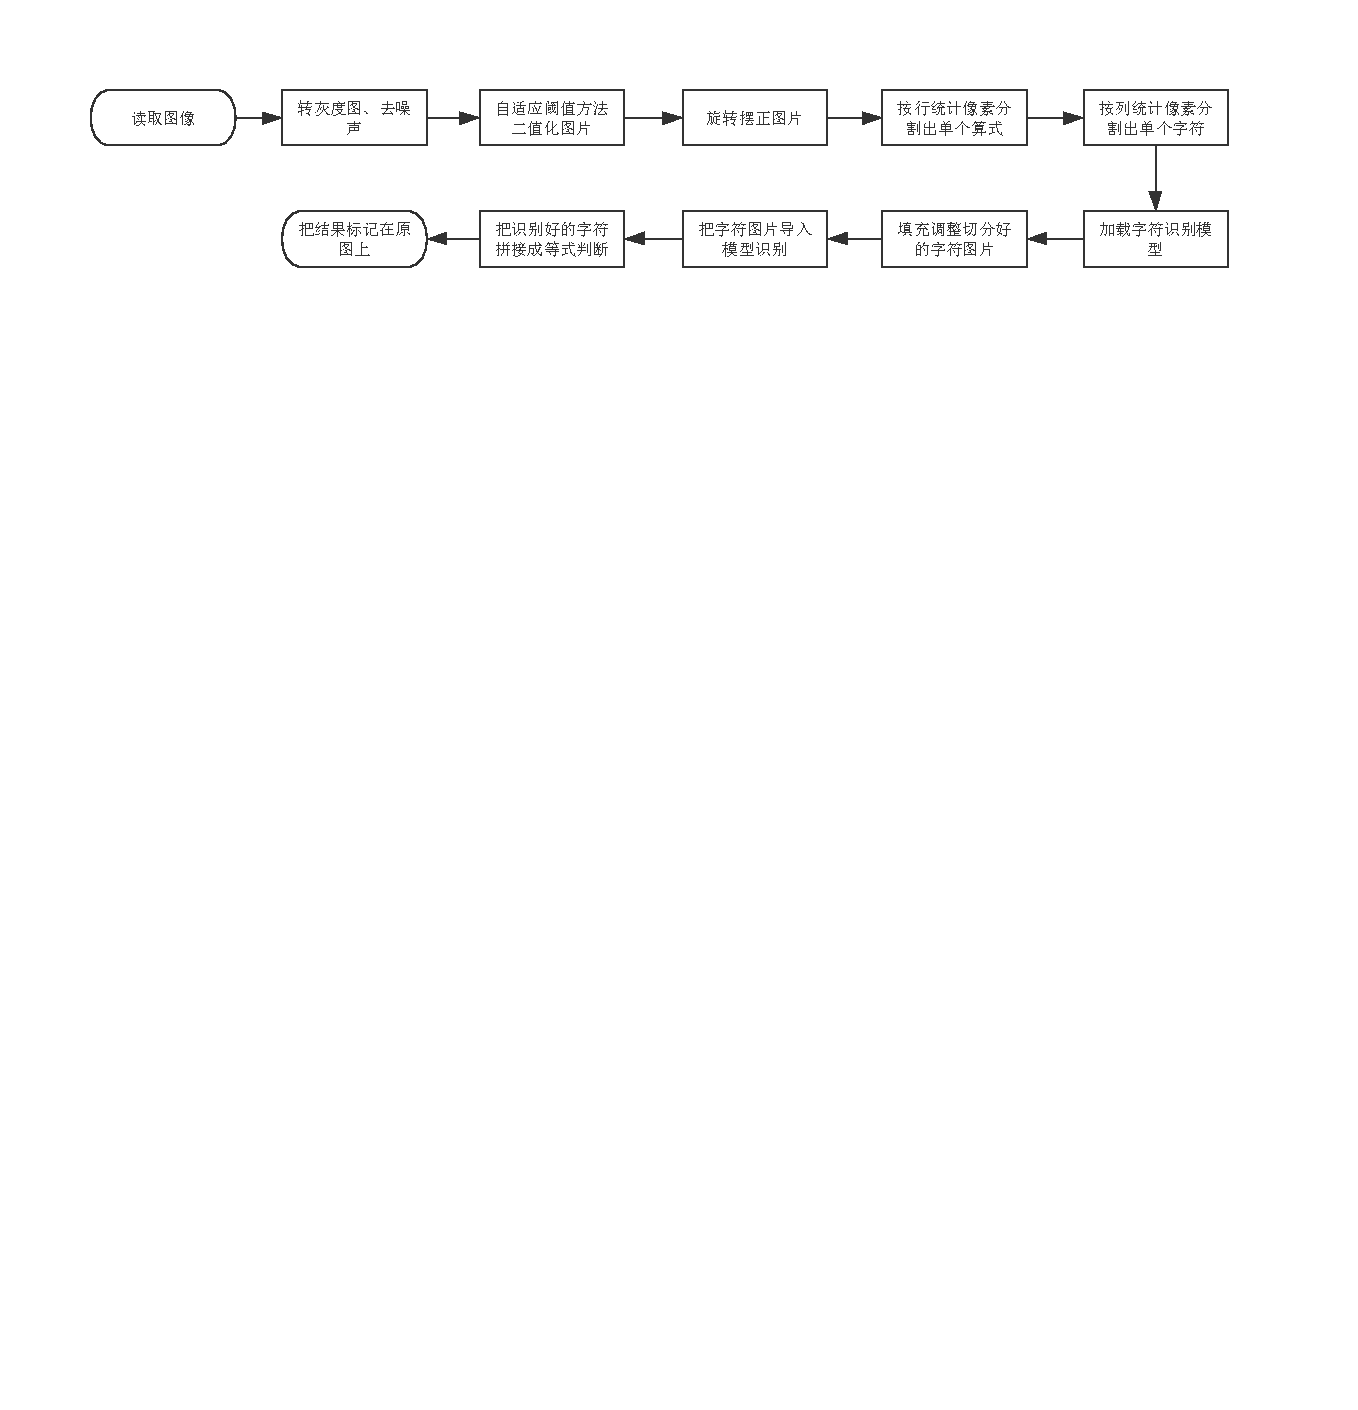
\includegraphics[width=350bp]{picture/cut.pdf}
	\caption{识别步骤}
	\label{fig:}
\end{figure}
\par

\section{基于ResNet18的字符识别模型}
\subsection{数据集的预处理}
本模型的数据集由minist数据集和手写运算符组成,数字图片来自minist数据集,图片大小为28*28,运算符数据集来自kaggle,图片大小为45*45。首先需要把没有规律的图片名称改为按数字递增,方便划分训练集、测试集和加载到神经网络。运算符图片的大小为45*45,且图片内的字符接触图片边缘,而本文从整张图片中切分出的字符图片内的字符与图片边缘不相交,所以需要填充图片边缘后再调整大小。将运算符图片的上下左右边缘各填充10个像素变为65*65,然后调整大小为28*28。
\subsection{训练模型}
训练集共有60000张数字图片和加、减、乘、除、等号、左右括号每种运算符5000张;测试集中有10000张数字图片和10500张运算符图片,每种运算符占1500张,将手写运算符拼接到minist数据集后打乱顺序后导入残差网络训练。使用随机梯度下降算法进行训练优化,初始学习率设为0.1,每30轮降低10\%的学习率,冲量参数设为0.9,权重衰减设为5e-4。导入到ResNet18后训练90轮后在测试集上的识别准确率为99.776\%。
\begin{figure}[h!]
	\centering
	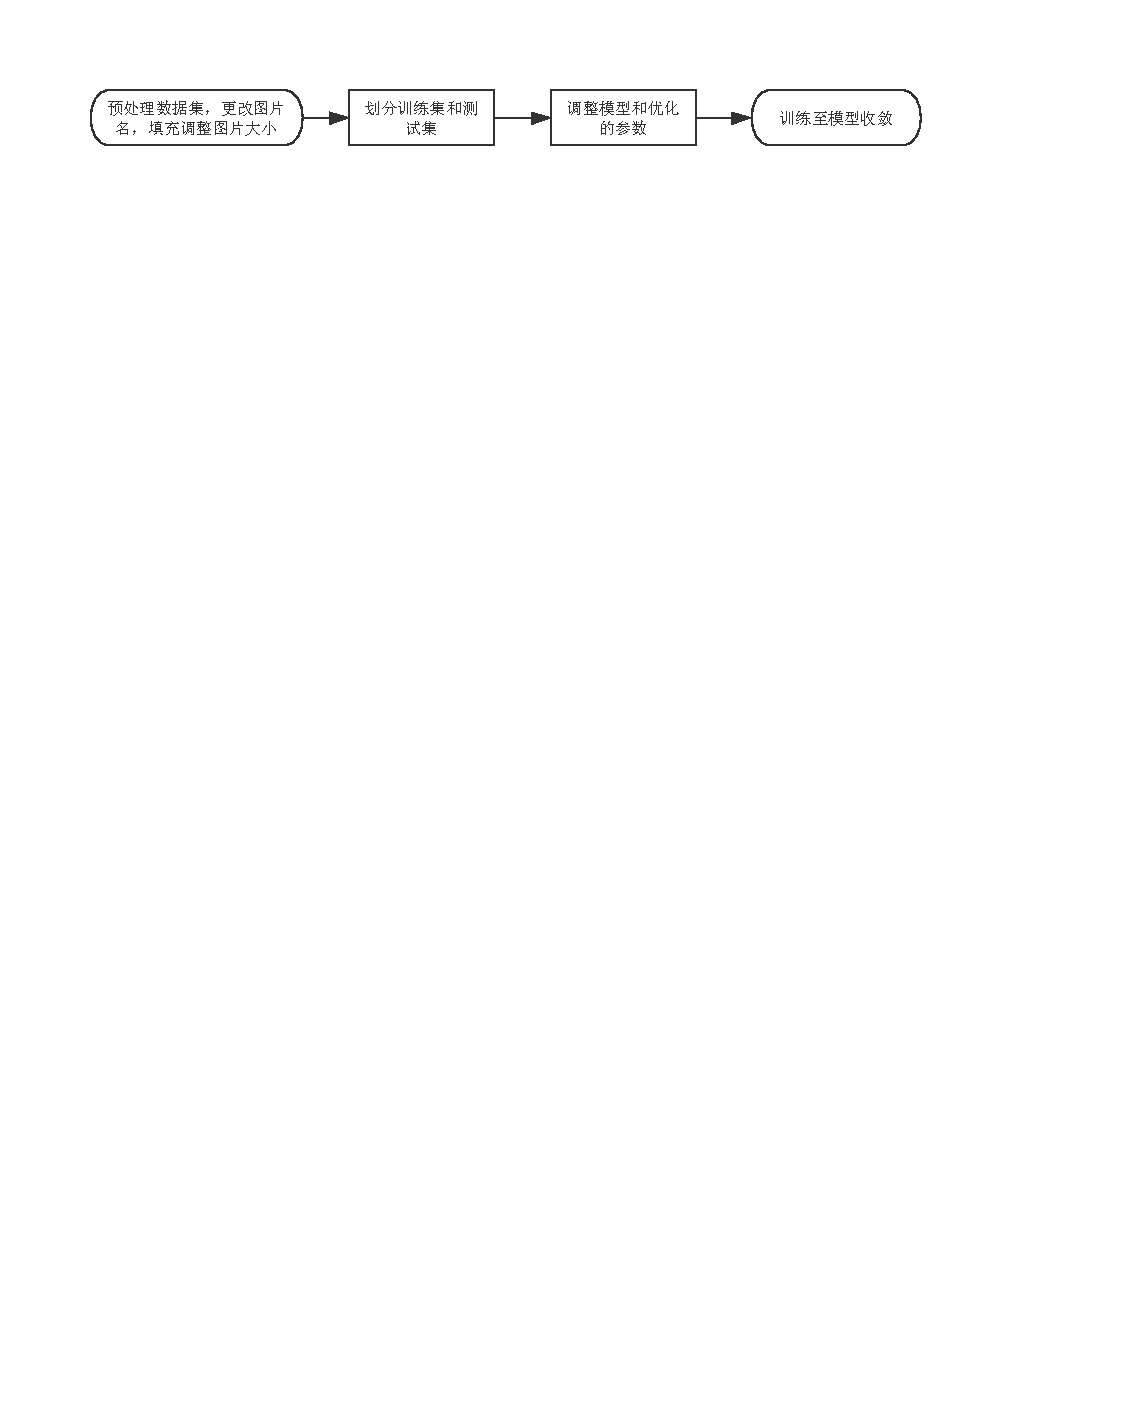
\includegraphics[width=350bp]{picture/train.pdf}
	\caption{训练步骤}
	\label{fig:}
\end{figure}
\par

\section{本章小结}
